\documentclass[a4paper,11pt]{article}
\usepackage[a4paper, margin=8em]{geometry}

% usa i pacchetti per la scrittura in italiano
\usepackage[french,italian]{babel}
\usepackage[T1]{fontenc}
\usepackage[utf8]{inputenc}
\frenchspacing 

% usa i pacchetti per la formattazione matematica
\usepackage{amsmath, amssymb, amsthm, amsfonts}

% usa altri pacchetti
\usepackage{gensymb}
\usepackage{hyperref}
\usepackage{standalone}

\usepackage{colortbl}

\usepackage{xstring}
\usepackage{karnaugh-map}

% imposta il titolo
\title{Appunti Sistemi Operativi}
\author{Luca Seggiani}
\date{2025}

% imposta lo stile
% usa helvetica
\usepackage[scaled]{helvet}
% usa palatino
\usepackage{palatino}
% usa un font monospazio guardabile
\usepackage{lmodern}

\renewcommand{\rmdefault}{ppl}
\renewcommand{\sfdefault}{phv}
\renewcommand{\ttdefault}{lmtt}

% circuiti
\usepackage{circuitikz}
\usetikzlibrary{babel}

% testo cerchiato
\newcommand*\circled[1]{\tikz[baseline=(char.base)]{
            \node[shape=circle,draw,inner sep=2pt] (char) {#1};}}

% disponi il titolo
\makeatletter
\renewcommand{\maketitle} {
	\begin{center} 
		\begin{minipage}[t]{.8\textwidth}
			\textsf{\huge\bfseries \@title} 
		\end{minipage}%
		\begin{minipage}[t]{.2\textwidth}
			\raggedleft \vspace{-1.65em}
			\textsf{\small \@author} \vfill
			\textsf{\small \@date}
		\end{minipage}
		\par
	\end{center}

	\thispagestyle{empty}
	\pagestyle{fancy}
}
\makeatother

% disponi teoremi
\usepackage{tcolorbox}
\newtcolorbox[auto counter, number within=section]{theorem}[2][]{%
	colback=blue!10, 
	colframe=blue!40!black, 
	sharp corners=northwest,
	fonttitle=\sffamily\bfseries, 
	title=Teorema~\thetcbcounter: #2, 
	#1
}

% disponi definizioni
\newtcolorbox[auto counter, number within=section]{definition}[2][]{%
	colback=red!10,
	colframe=red!40!black,
	sharp corners=northwest,
	fonttitle=\sffamily\bfseries,
	title=Definizione~\thetcbcounter: #2,
	#1
}

% disponi codice
\usepackage{listings}
\usepackage[table]{xcolor}

\definecolor{codegreen}{rgb}{0,0.6,0}
\definecolor{codegray}{rgb}{0.5,0.5,0.5}
\definecolor{codepurple}{rgb}{0.58,0,0.82}
\definecolor{backcolour}{rgb}{0.95,0.95,0.92}

\lstdefinestyle{codestyle}{
		backgroundcolor=\color{black!5}, 
		commentstyle=\color{codegreen},
		keywordstyle=\bfseries\color{magenta},
		numberstyle=\sffamily\tiny\color{black!60},
		stringstyle=\color{green!50!black},
		basicstyle=\ttfamily\footnotesize,
		breakatwhitespace=false,         
		breaklines=true,                 
		captionpos=b,                    
		keepspaces=true,                 
		numbers=left,                    
		numbersep=5pt,                  
		showspaces=false,                
		showstringspaces=false,
		showtabs=false,                  
		tabsize=2
}

\lstdefinestyle{shellstyle}{
		backgroundcolor=\color{black!5}, 
		basicstyle=\ttfamily\footnotesize\color{black}, 
		commentstyle=\color{black}, 
		keywordstyle=\color{black},
		numberstyle=\color{black!5},
		stringstyle=\color{black}, 
		showspaces=false,
		showstringspaces=false, 
		showtabs=false, 
		tabsize=2, 
		numbers=none, 
		breaklines=true
}


\lstdefinelanguage{assembler}{ 
  keywords={AAA, AAD, AAM, AAS, ADC, ADCB, ADCW, ADCL, ADD, ADDB, ADDW, ADDL, AND, ANDB, ANDW, ANDL,
        ARPL, BOUND, BSF, BSFL, BSFW, BSR, BSRL, BSRW, BSWAP, BT, BTC, BTCB, BTCW, BTCL, BTR, 
        BTRB, BTRW, BTRL, BTS, BTSB, BTSW, BTSL, CALL, CBW, CDQ, CLC, CLD, CLI, CLTS, CMC, CMP,
        CMPB, CMPW, CMPL, CMPS, CMPSB, CMPSD, CMPSW, CMPXCHG, CMPXCHGB, CMPXCHGW, CMPXCHGL,
        CMPXCHG8B, CPUID, CWDE, DAA, DAS, DEC, DECB, DECW, DECL, DIV, DIVB, DIVW, DIVL, ENTER,
        HLT, IDIV, IDIVB, IDIVW, IDIVL, IMUL, IMULB, IMULW, IMULL, IN, INB, INW, INL, INC, INCB,
        INCW, INCL, INS, INSB, INSD, INSW, INT, INT3, INTO, INVD, INVLPG, IRET, IRETD, JA, JAE,
        JB, JBE, JC, JCXZ, JE, JECXZ, JG, JGE, JL, JLE, JMP, JNA, JNAE, JNB, JNBE, JNC, JNE, JNG,
        JNGE, JNL, JNLE, JNO, JNP, JNS, JNZ, JO, JP, JPE, JPO, JS, JZ, LAHF, LAR, LCALL, LDS,
        LEA, LEAVE, LES, LFS, LGDT, LGS, LIDT, LMSW, LOCK, LODSB, LODSD, LODSW, LOOP, LOOPE,
        LOOPNE, LSL, LSS, LTR, MOV, MOVB, MOVW, MOVL, MOVSB, MOVSD, MOVSW, MOVSX, MOVSXB,
        MOVSXW, MOVSXL, MOVZX, MOVZXB, MOVZXW, MOVZXL, MUL, MULB, MULW, MULL, NEG, NEGB, NEGW,
        NEGL, NOP, NOT, NOTB, NOTW, NOTL, OR, ORB, ORW, ORL, OUT, OUTB, OUTW, OUTL, OUTSB, OUTSD,
        OUTSW, POP, POPL, POPW, POPB, POPA, POPAD, POPF, POPFD, PUSH, PUSHL, PUSHW, PUSHB, PUSHA, 
				PUSHAD, PUSHF, PUSHFD, RCL, RCLB, RCLW, MOVSL, MOVSB, MOVSW, STOSL, STOSB, STOSW, LODSB, LODSW,
				LODSL, INSB, INSW, INSL, OUTSB, OUTSL, OUTSW
        RCLL, RCR, RCRB, RCRW, RCRL, RDMSR, RDPMC, RDTSC, REP, REPE, REPNE, RET, ROL, ROLB, ROLW,
        ROLL, ROR, RORB, RORW, RORL, SAHF, SAL, SALB, SALW, SALL, SAR, SARB, SARW, SARL, SBB,
        SBBB, SBBW, SBBL, SCASB, SCASD, SCASW, SETA, SETAE, SETB, SETBE, SETC, SETE, SETG, SETGE,
        SETL, SETLE, SETNA, SETNAE, SETNB, SETNBE, SETNC, SETNE, SETNG, SETNGE, SETNL, SETNLE,
        SETNO, SETNP, SETNS, SETNZ, SETO, SETP, SETPE, SETPO, SETS, SETZ, SGDT, SHL, SHLB, SHLW,
        SHLL, SHLD, SHR, SHRB, SHRW, SHRL, SHRD, SIDT, SLDT, SMSW, STC, STD, STI, STOSB, STOSD,
        STOSW, STR, SUB, SUBB, SUBW, SUBL, TEST, TESTB, TESTW, TESTL, VERR, VERW, WAIT, WBINVD,
        XADD, XADDB, XADDW, XADDL, XCHG, XCHGB, XCHGW, XCHGL, XLAT, XLATB, XOR, XORB, XORW, XORL},
  keywordstyle=\color{blue}\bfseries,
  ndkeywordstyle=\color{darkgray}\bfseries,
  identifierstyle=\color{black},
  sensitive=false,
  comment=[l]{\#},
  morecomment=[s]{/*}{*/},
  commentstyle=\color{purple}\ttfamily,
  stringstyle=\color{red}\ttfamily,
  morestring=[b]',
  morestring=[b]"
}

\lstset{language=assembler, style=codestyle}

% disponi sezioni
\usepackage{titlesec}

\titleformat{\section}
	{\sffamily\Large\bfseries} 
	{\thesection}{1em}{} 
\titleformat{\subsection}
	{\sffamily\large\bfseries}   
	{\thesubsection}{1em}{} 
\titleformat{\subsubsection}
	{\sffamily\normalsize\bfseries} 
	{\thesubsubsection}{1em}{}

% tikz
\usepackage{tikz}

% float
\usepackage{float}

% grafici
\usepackage{pgfplots}
\pgfplotsset{width=10cm,compat=1.9}

% disponi alberi
\usepackage{forest}

\forestset{
	rectstyle/.style={
		for tree={rectangle,draw,font=\large\sffamily}
	},
	roundstyle/.style={
		for tree={circle,draw,font=\large}
	}
}

% disponi algoritmi
\usepackage{algorithm}
\usepackage{algorithmic}
\makeatletter
\renewcommand{\ALG@name}{Algoritmo}
\makeatother

% disponi numeri di pagina
\usepackage{fancyhdr}
\fancyhf{} 
\fancyfoot[L]{\sffamily{\thepage}}

\makeatletter
\fancyhead[L]{\raisebox{1ex}[0pt][0pt]{\sffamily{\@title \ \@date}}} 
\fancyhead[R]{\raisebox{1ex}[0pt][0pt]{\sffamily{\@author}}}
\makeatother

\begin{document}
% sezione (data)
\section{Lezione del 30-09-25}

% stili pagina
\thispagestyle{empty}
\pagestyle{fancy}

% testo
Continuiamo la discussione della memoria RAM.

Avevamo introdotto il meccanismo della cache come una sorta di "memoizzazione" dei dati in occasione del primo accesso.
In verità, nei moderni processori (dal Pentium in poi) abbiamo due cache separate:
\begin{itemize}
	\item La \textbf{I-cache}, cioè \textit{cache istruzioni};
	\item La \textbf{D-cache}, cioè \textit{cache dati};
\end{itemize}

Il vantaggio di distinguere fra cache istruzioni e cache dati è che la I-cache enon ha bisongo di essere ricopiata in memoria alla fine dell'utilizzo, e probabilmente deve mantenere zone di memoria molto specifiche, per cui ha senso non rallentarne l'operazione chiedendole di mantenere anche informazioni sui dati.

\subsubsection{Gerarchie di memoria}
Fra registri, RAM, dispositivi a blocchi, ecc... abbiamo visto diverse fonti di \textit{memoria} che un calcolatore può utilizzare. Potrebbe avere senso organizzare queste memorie in una struttura gerarchica, magari per \textit{dimensione crescente} in avanti (e di conseguenza per \textit[velocità] all'indietro):
\begin{enumerate}
	\item Registri interni;
	\item Cache;
	\item RAM;
	\item Dischi;
	\item Nastri.
\end{enumerate}

\subsection{Schema a blocchi di un semplice calcolatore}
Possiamo quindi, dopo aver visto tutte le componenti che lo compongono, vedere lo schema a blocchi di un semplice calcolatore: 

\begin{center}
	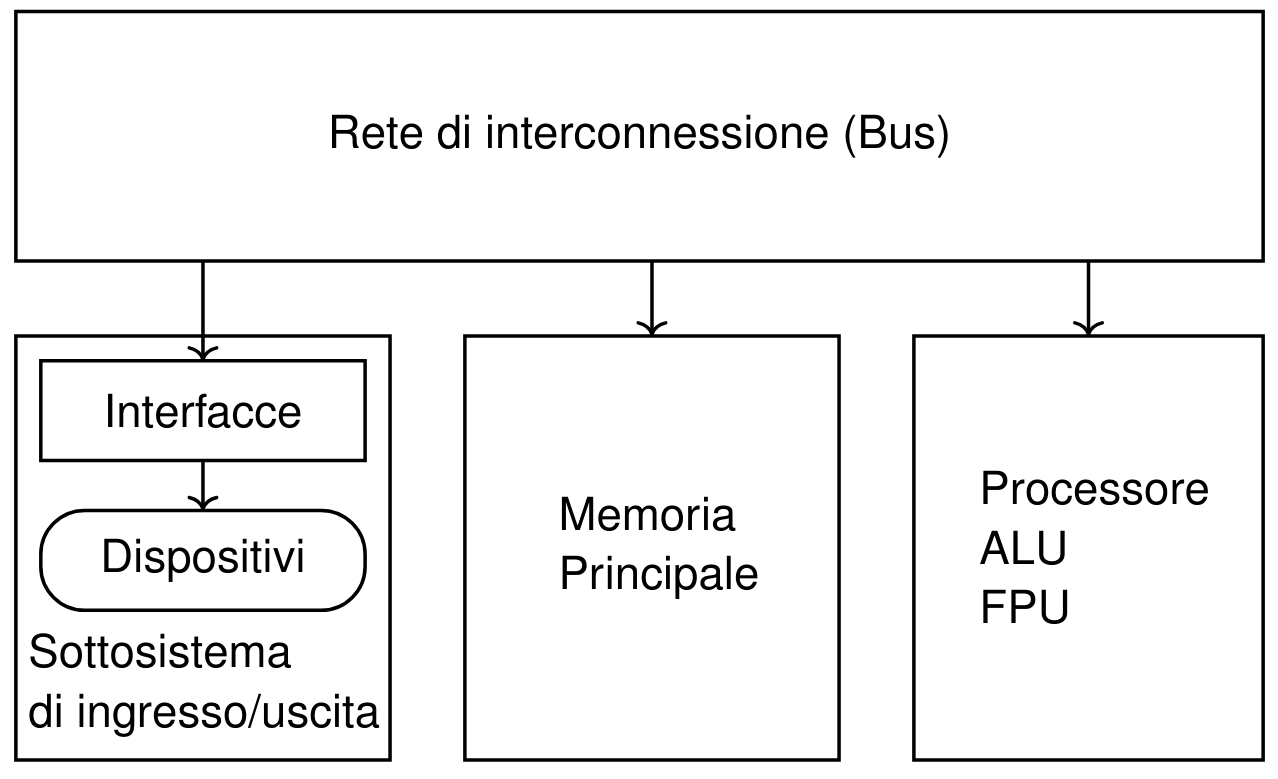
\includegraphics[scale=0.35]{../figures/struttura_calc.png}
\end{center}

Vediamo quindi come questi componenti comunicano fra di loro:
\begin{itemize}
	\item La rete di interconnessione (bus) serve tutti (a scapito della direzione delle frecce, può supportare la comunicazione \textit{da} e \textit{a} componenti);
	\item Il processore e la RAM si trovano sul bus;
	\item I dispositivi, cioè i trasduttori col mondo esterno, comunicano con il sistema attraverso le loro \textit{interfacce}, che obbedisce da un lato alle regole del bus e dall'altro alle specifiche del dispositivo stesso per permettere la comunicazione.
\end{itemize}

\subsection{Interfacce}
Abbiamo visto come fra il calcolatore ed ogni dispositivo si trovi un'apposita \textit{interfaccia}.

Di base, ogni interfaccia è caratterizzata da più registri (accessibili nello spazio di I/O), che possono essere scritti o letti dal calcolatore per dare o ottenere informazioni dal dispositivo.
Notiamo che letture e scritture sui registri delle interfacce possono essere distruttive: spesso il dispositivo implementa particolari funzioni che vengono lanciate da operazioni di questo tipo (un registro che si azzera dopo esser letto, ecc...).

Nel caso più semplice, in ogni caso, un'interfaccia dispone di almeno 3 registri:
\begin{itemize}
	\item Registro di \textbf{stato}, che segnala lo stato corrente dell'interfaccia (se è di uscita può segnalare che è pronta a ricevere dati, se di entrata che ci sono dati pronti, ecc...);
	\item Registro di \textbf{controllo}, che permette al calcolatore di comandarne l'operazione (se di entrata può impedire che nuovi dati arrivino in ingresso, ecc...);
	\item Uno o più \textbf{buffer dati}, resi accessibili attraverso un registro di lettura. Solitamente si dice \textbf{TBR} (\textit{Transfer Buffer Register}) il registro che accede al buffer di uscita e \textbf{RBR} (\textit{Receive Buffer Register}) il registro che accede al buffer di entrata. Nel caso di interfacce di ingresso/uscita TBR e RBR stanno alla stessa porta dello spazio di I/O, e quale viene reso disponibile al processore varia in base al tipo di operazione che esso richiede (TBR per uscita, RBR per ingresso).
\end{itemize}

\subsection{Interruzioni}
Veniamo quindi al meccanismo dell'\textbf{interruzione}.
Nella formulazione originale di Dijkstra queste servivano a risparmiare al processore l'attesa "attiva" (\textit{busy wait}) dei bit di stato delle interfacce, delegando questo invece ad una segnalazione esplicita da parte dell'interfaccia, che viene \textit{gestita} dal processore mettendo in esecuzione un determinato \textit{handler} di interruzione.

Per gestire correttamente le interruzioni abbiamo bisogno di un po' di infrastruttura in più:
\begin{itemize}
	\item Una nuova fase processore, successiva all'esecuzione, che si occupa di controllare le richieste di interruzioni in arrivo (nei sistemi x86 \textit{la} richiesta, che è stata inoltrata da un sottosistema detto APIC);
	\item Una zona di memoria dove viene allocata la \textbf{IVT} (\textit{Interrupt Vector Table}), che associa ad un indice (cioè il tipo di interruzione) l'inizio dell'handler relativo a tale tipo;
	\item Una nuova istruzione, \lstinline|IRET|, che si occupa di ritornare da un gestore di interruzione.

		Non potremmo usare la semplice RET in quanto ogni interruzione salva dello stato aggiuntivo oltre al semplice IP sulla pila: di base, salveremo anche il registro dei FLAG.
\end{itemize}

\subsubsection{Tipi di interruzione}
Abbiamo visto nel corso di calcolatori elettronici come il meccanismo delle interruzioni può essere sfruttato per implementare molta più funzionalità di quelle relative alla gestione dei dispositivi.
In particolare, i calcolatori moderni dispongono di più tipi di interruzioni:
\begin{itemize}
	\item Interruzioni \textbf{esterne}, del tipo che abbiamo appena visto, che si distinguono ulteriormente in:
		\begin{itemize}
			\item Interruzioni esterne \textbf{mascherabili}, cioè che possono essere ignorate variando il flag IF;
			\item Interruzioni esterne \textbf{non mascherabili}, cioè che vengono sempre gestite;
		\end{itemize}
	\item Interruzioni \textbf{interne}, cioè lanciate da situazioni interne al processore (eccezioni);
	\item Interruzioni \textbf{software}, che possono essere lanciate dal programmatore attraverso l'apposita istruzione \lstinline|INT|.
\end{itemize}

\subsection{Meccanismi di protezione}
Veniamo quindi ai meccanismi tipici del S/O in sé per sé.
Se vogliamo la separazione fra processi e S/O che gestisce quei processi (e quindi ha l'accesso prioritario alle risorse di sistema), dobbiamo separare l'operazione del calcolatore in due modalità principali:
\begin{itemize}
	\item Modalità \textbf{utente}: usata per la normale esecuzione dei programmi, non è possibile accedere a tutte le risorse di sistema;
	\item Modalità \textbf{supervisor}: usata per lo svolgimento delle chiamate sistema (primitive), tutte le risorse di sistema sono disponibili.
\end{itemize}

Importante è che il passaggio da modo utente a modo supervisor richieda al programma in esecuzione in modo utente di "abbandonare" il controllo, cedendolo ad una primitiva sistema.
Vedremo come questo si può implementare agilmente sfruttando il meccanismo di interruzione.

\subsection{Componenti del S/O}
Vediamo quindi, come abbiamo fatto per l'hardware, quelli che sono i \textbf{componenti} del S/O e come questi sono organizzati.

Prendiamo come riferimento un sistema \textit{Unix}, in quanto più semplice ed elegante per i nostri scopi.

Adottando un approccio \textit{top-down}, dove per \textit{top} intendiamo lo spazio dell'utente, vediamo le seguenti componenti:
\begin{itemize}
	\item L'\textit{userspace}, cioè gli applicativi utente veri e propri;
	\item Gli strumenti che il S/O fornisce all'utente per la gestione del sistema, cioè:
		\begin{itemize}
			\item La \textbf{shell};
			\item \textbf{Compilatore} e \textbf{linker};
			\item Le \textbf{librerie} sistema (che si rivolgono ad API, ecc...).
		\end{itemize}
	\item Il \textbf{kernel}, cioè la parte del S/O che effettivamente gestisce il sistema. Qui troviamo:
		\begin{itemize}
			\item Il sottosistema \textbf{file}, che gestisce il filesystem su uno o più dispositivi a blocchi;
			\item A sua volta il sottosistema file interagisce con i \textbf{driver} dispositivo (in particolare coi driver dei dispositivi a blocchi), che hanno il compito di gestire a livello hardware il comportamento dei dispositivi;
			\item Inoltre, troviamo il sottosistema \textbf{controllo processi}, composto da:
				\begin{itemize}
					\item Funzionalità \textbf{IPC} (\textit{Inter Process Communication}) per la comunicazione fra processi;
					\item Lo \textbf{scheduler}, che decide quali processi mandare in esecuzione;
					\item Il sottosistema di \textbf{gestione memoria}, che gestisce lo spazio in memoria principale allocato per ogni processo, interagendo col meccanismo della \textit{memoria virtuale}.
				\end{itemize}
		\end{itemize}
	\item Infine, il \textit{kernel} si appoggia all'\textbf{hardware} della macchina. 
\end{itemize}

\subsubsection{Modello gerarchico}
Un modello più complesso per S/O potrebbe elaborare su questa struttura, prevedendo più livelli intermedi di kernel che implementano \textit{macchine virtuali} via via più vicine all'hardware.
Ognuna di queste fornirà al livello superiore funzioni (effettivamente chiamate sistema) sempre più astratte, che implementeranno nel complesso le chiamate sistema rese disponibili ai processi utente.

\subsubsection{Modello client-server}
Un'altro modello possibile per sistemi distribuiti in rete è quello di avere più \textit{nodi} collegati alla stessa rete.
Ogni nodo disporrà del suo kernel, e in esecuzione su quel kernel avrà uno specifico processo (utente o sistema).

La funzionalità del S/O sarà quindi implementata interrogando la rete per il servizio richiesto: sarà quindi compito della macchina su quella rete che effettivamente implementa tale servizio rispondere e fornire, appunto, il servizio.

In ogni caso non analizzeremo sistemi di questo tipo in questo corso, relativi più che altro a sistemi su \textit{cloud}, e quindi all'ambito delle reti informatiche.

\subsection{Gestione dei processi}
Informalmente, il termine processo viene usato per indicare un programma in esecuzione sulla macchina.

\begin{itemize}
	\item Rappresenta la \textit{sequenza di eventi} generati dall'elaboratore durante l'esecuzione;
	\item Identifica la più piccola \textit{unità di esecuzione} dentro un S/O multiprogrammato: questo consentirà l'esecuzione di \textit{più} processi concorrenti;
\end{itemize}

Un processo va necessariamente \textit{descritto}, cioè bisogna definire un \textbf{descrittore} che lo rappresenta.
Del processo ci interessa:
\begin{itemize}
	\item Il \textbf{codice} del programma che esegue;
	\item I \textbf{dati};
	\item Il valore dell'\textbf{IP};
	\item Lo stato dei \textbf{registri};
	\item Lo \textbf{stack}.
\end{itemize}

Inoltre, ad un certo processo potranno essere associate delle risorse:
\begin{itemize}
	\item \textbf{Memoria} utilizzata;
	\item \textbf{File} aperti;
	\item \textbf{Dispositivi} di I/O a cui ha accesso.
\end{itemize}

\subsubsection{Processi in memoria}
Il processo in memoria ha a disposizione il suo \textit{spazio di indirizzamento virtuale}. 
Viene detto \textit{virtuale} perché verrà allocato in una memoria centrale fisica, le cui locazioni potrebbero non corrispondere esattamente con la memoria offerta al processo (attraverso il meccanismo della \textit{memoria virtuale}).

Partendo dal basso, le regioni di memoria fornite al processo nel suo spazio di indirizzamento saranno:
\begin{enumerate}
	\item \lstinline|text|: contiene il codice del processo;
	\item \lstinline|data|: contiene i dati statici del programa (sezione \lstinline|data| e \lstinline|bss|, che contiene lo spazio riservato a variabili statiche non allocate);
	\item \lstinline|heap|: l'heap del processo, dove vengono allocati oggetti in memoria dinamica; 
	\item \lstinline|stack|: si sviluppa verso il basso, rappresenta la pila del processo in esecuzione.
\end{enumerate}

\end{document}
